\chapter{Application to Fashion-MNIST inverted}\label{ch:part-c}

\section{Motivation}\label{sec:part-c-motivation}

In this section, we interpret the requirement of applying the method to a different problem: the method is SR-FCA, and a ``different problem'' means changing either the dataset or the source of client heterogeneity. In Chapter~\ref{ch:experiments} we already swapped the dataset (MNIST $\to$ Fashion-MNIST) while keeping the heterogeneity source (rotation). Here we swap the heterogeneity source: the dataset is Fashion-MNIST again, but the clients are split by \emph{pixel inversion} rather than rotation. The question we answer is:

\begin{quote}
    \itshape Does the clustering primitive inside SR-FCA work regardless of the physical cause of heterogeneity, or does it depend on the specific geometry of the image-space transform?
\end{quote}

Rotation by a cardinal angle and pixel-inversion $x \mapsto 1-x$ induce very different changes in the MLP's weight space: the first is a spatial transform that a shallow MLP can only partially compensate, while the second is a per-pixel affine transform that the first hidden layer can absorb almost exactly. If the clustering signal was specific to the rotation geometry, we would expect SR-FCA to under-perform on inversion.

\section{Setup}\label{sec:part-c-setup}

Everything carries over from Chapter~\ref{ch:experiments}: $m = 100$ clients, $n = 600$ samples per client, 2-layer MLP (hidden $= 200$), and the paper's full-scale SR-FCA configuration ($T = 280$, $E = 2$, $R = 2$, $\beta = 0.1$). Five seeds. The only differences from the MNIST setup are \texttt{dataset="fashion\_mnist"} and \texttt{split="inverted"} in the data loader, and $K^\star = 2$ (identity vs.\ pixel-inverted).

We run SR-FCA only -- the same scope decision as Chapter~\ref{ch:experiments}. The histogram heuristic picks $\lambda$ once at seed~$0$ from the pairwise-$\ell_2$ histogram, then is reused for the remaining four seeds.

\section{Results}\label{sec:part-c-results}

\begin{figure}[h]
\centering
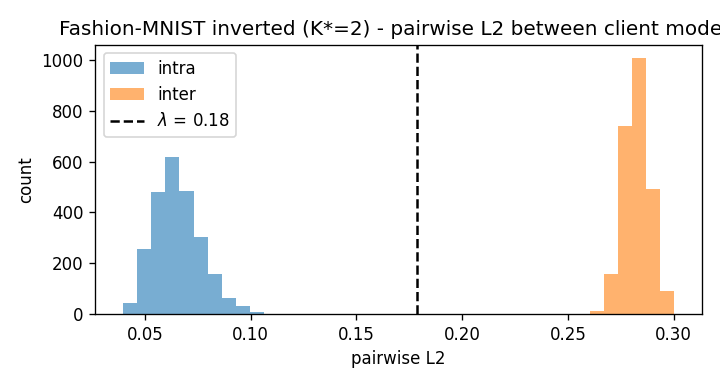
\includegraphics[width=0.49\textwidth]{Figures/srfca/pairwise_hist_part_c.png}
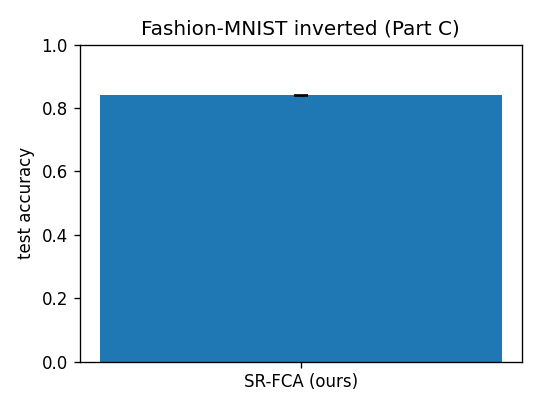
\includegraphics[width=0.49\textwidth]{Figures/srfca/part_c_bar.png}
\caption{Left: pairwise-$\ell_2$ histogram on Fashion-MNIST inverted (seed~$0$, $K^\star = 2$). Right: test accuracy of SR-FCA across five seeds.}\label{fig:part-c}
\end{figure}

\begin{table}[h]
\centering
\small
\begin{tabular}{lcc}
\toprule
Method & Test acc (\%) & Misclust. \\
\midrule
\textbf{SR-FCA} & $\mathbf{84.00 \pm 0.22}$ & $\mathbf{0.00}$ \\
\bottomrule
\end{tabular}
\caption{Fashion-MNIST \emph{inverted} (Part C), five seeds, full-scale SR-FCA configuration.}\label{tab:part-c}
\end{table}

\paragraph{Pairwise-distance histogram.} The histogram on Fashion-MNIST inverted (Figure~\ref{fig:part-c}, left) is cleanly bimodal: intra-cluster distances concentrate on the left mode, inter-cluster distances on the right, with a narrow valley between. The histogram heuristic picks $\lambda$ on the first try, exactly as on MNIST.

\paragraph{Cluster recovery.} SR-FCA recovers $K^\star = 2$ with zero misclustering on every seed of the five-seed run. Test accuracy is $84.00 \pm 0.22\,\%$ -- essentially indistinguishable from the rotated-split accuracy of $83.96 \pm 0.30\,\%$ in \S\ref{sec:fashion}, despite a fundamentally different heterogeneity source.

\section{Discussion}\label{sec:part-c-discussion}

The motivating question -- \emph{is the clustering primitive agnostic to the physical cause of heterogeneity?} -- is answered in the affirmative. SR-FCA reaches the same accuracy band on Fashion-MNIST inverted as on Fashion-MNIST rotated, with the same zero-misclustering cluster recovery on every seed. What SR-FCA actually detects is a \emph{functional} difference between clients: two clients sharing a task produce similar local models, two clients with different tasks produce dissimilar ones, and the pairwise-distance histogram is the right object to quantify this regardless of whether the task difference was induced by rotation, inversion, or something else.

The fact that rotation ($K^\star = 4$, four cardinal angles) and inversion ($K^\star = 2$, two pixel-affine transforms) produce essentially identical SR-FCA accuracy on Fashion-MNIST is empirically reassuring. The two heterogeneity sources are mathematically very different -- a spatial transform that the MLP can only partially compensate, versus a per-pixel affine transform that the first hidden layer can absorb almost exactly -- yet SR-FCA's clustering primitive is sensitive enough to separate clients in either regime. This is consistent with the paper's motivating examples (keyboard-typing languages, hospital specialities) and adds an empirical data point on a second, orthogonal axis of heterogeneity.

A natural extension is to test a \emph{compositional} heterogeneity source: some clients rotated, some inverted, some both, with $K^\star = 4$ derived from the four transformation combinations. We expect SR-FCA to recover the correct clustering (the four combinations induce four distinguishable functional behaviours), but the histogram would have three modes and the valley heuristic would need to be replaced by a multi-threshold procedure. We leave this to follow-up work.
